\section{Target users analysis}\label{sec:target-users-analysis}

When working on a large scale project, it is important to analyze who the target user-base is.
The problem has to be big enough to affect numerous users and the solution has to be viable to be used by said
users.

\subsection{Users}\label{subsec:users}

The main issue is about travelling, which covers a wide range of people, as almost everyone travels one way or
another.
Some examples include travelling to work, travelling to school, family visits, or outings with friends.
As this range is too broad we will in the following section narrow the target user-base down.
There are already some solution to this issue, but in Section~\ref{sec:extant-solutions-and-their-operational-mechanisms},
we figured that these already existing solutions are more fit for single trips, rather than every day travelling.
This gap in use case is mainly what we want to focus on, which is why our target audience is commuters.

\subsection{Age range}\label{subsec:age-range}

With our user group in mind, we can estimate an age range for commuters.
Commuting means to travel to the same destination and back on a regular basis.
Therefore, our focus on destinations for commuting are either education or work.

In Denmark, primary schools are chosen for students based on the district where the student lives~\cite{primary_school}.
This would exclude them from our target user-base, as we want to focus mostly on long distance commuters.
At shorter distances, we would need to exclude planes, trains, and for people younger than 18, cars, making it a matter
of whether the student should commute by walking or by bike, which are both \unit{CO_{2}} friendly options and trivial
to select between, making our solution somewhat irrelevant for this age group.

From secondary education however, students can freely pick which high school they want to go to and the closest school
will be assigned to them.
This, however, makes them a candidate for our user-base, as there are not as many high schools as there are primary.
Many students therefore have a longer commute to school.
Secondary education starts when the student is 16 years old~\cite{secondary_school}.
Our cutoff in the age range would be retirement, as we assume that retired individuals will no longer be commuting in
retirement.
The retirement age in Denmark is 66-68 years of age~\cite{retirement}, making our age range between 16 and 68 years.

The age range is rather large as the user-base includes a large part of the population, which makes our solution rather
difficult, as we have to accommodate it for teenagers as well as adults and the elderly.
The program will therefore have to tailored to all these age groups.

\subsection{Persona}\label{subsec:persona}

To further analyze our user-base, we decided to use the \textit{persona} method.
It works by creating fictional people with different fictional issues and look into how our solution could help them
with their issue.
We use these personas to get a better understanding of our target audience, which will help us in the design process.
Below are three personas, with their images generated by GAN AI~\cite{thispersondoesnotexist}, where each of them
cover different age groups and have distinct characteristics related to the main problem.

\renewcommand{\arraystretch}{1.5}

\noindent
\begin{figure}[H]
    \centering
    \begin{tabularx}{\textwidth}{ | l X | }
        \hline
        &                                               \\
        & 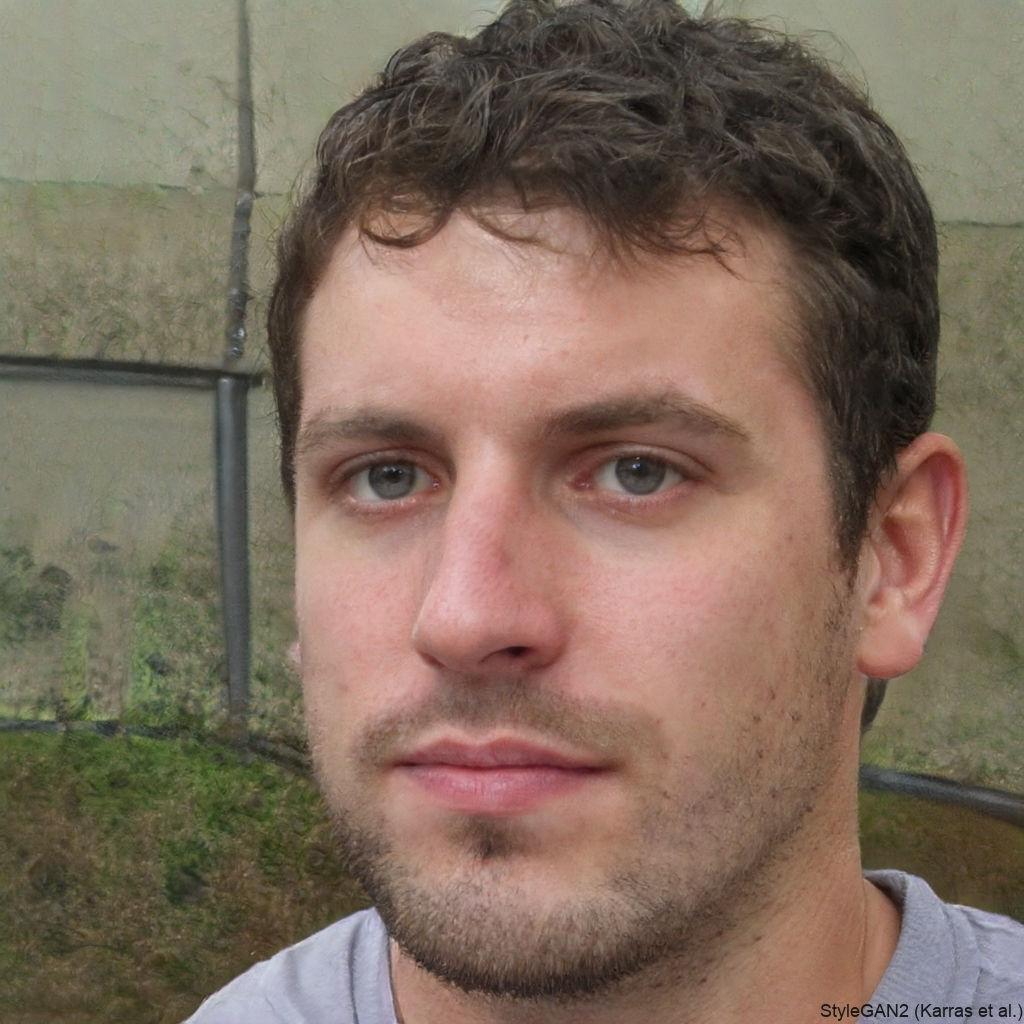
\includegraphics[width=0.25\textwidth]{asger} \\
        Name       & Asger Johansen                                \\
        Age        & 28 years old                                  \\
        Occupation & Designer                                      \\
        What's important & For Asger it is important to spend his days to the fullest.
        He is very outgoing, so he goes out with people after work.
        He hates having to stay overtime. \\
        Current problem & Asger just got a new job offer, but it's in another city.
        He isn't sure whether to move out or to commute there.
        He is also afraid of losing his free time if he has to travel. \\
        Potential solution & We would want to make a program, where Asger could calculate how long it'd take to commute from
        where he lives to the new job.
        He could compare different forms of transport and decide whether it's worth it to commute or if he should move out
        instead. \\
        \hline
    \end{tabularx}
    \caption{Persona: Asger.}
    % textidote: ignore begin
    \label{fig:persona_asger}
    % textidote: ignore end
\end{figure}

\noindent
\begin{figure}[H]
    \centering
    \begin{tabularx}{\textwidth}{ | l X | }
        \hline
        &                                                  \\
        & 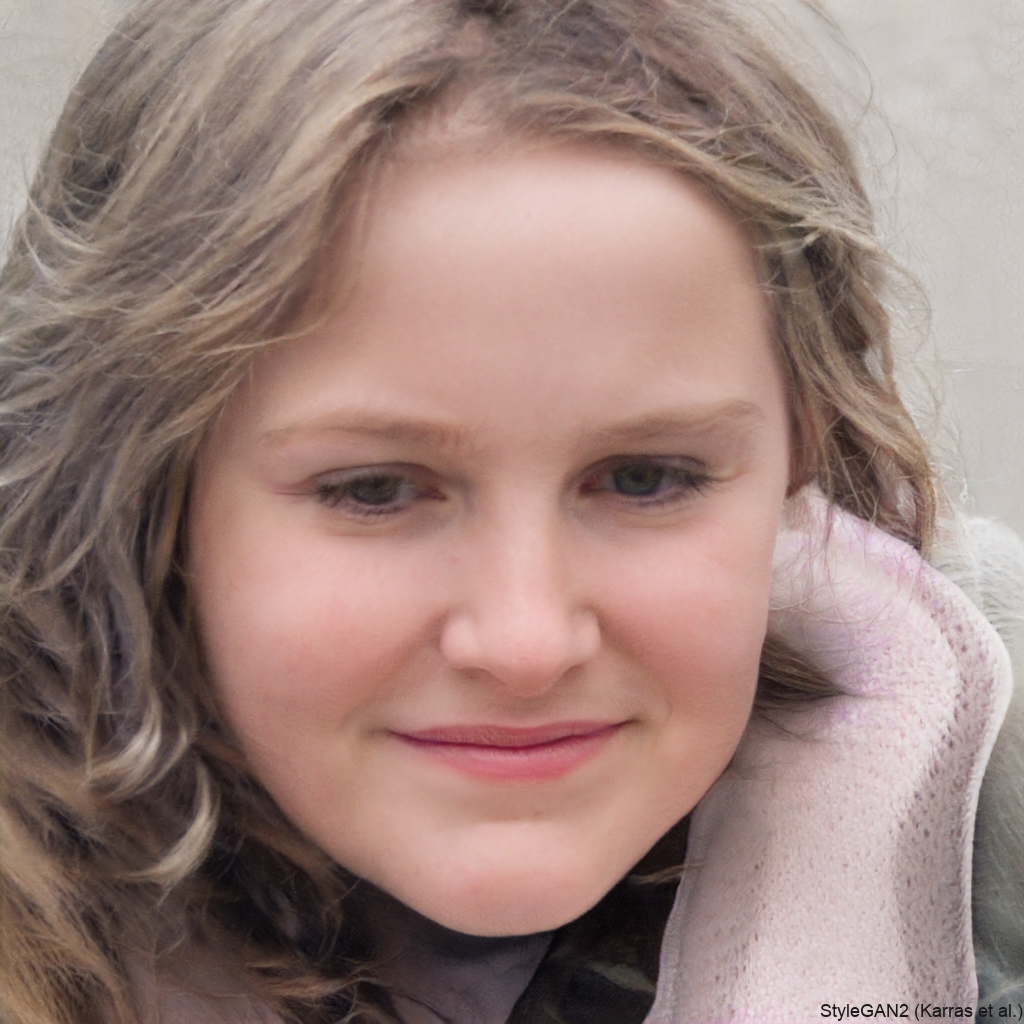
\includegraphics[width=0.25\textwidth]{josefine} \\
        Name       & Josefine Madsen                                  \\
        Age        & 19 years old                                     \\
        Occupation & Student                                          \\
        What's important & For Josefine, it is important to look after nature.
        She's been taught to think green since she was little, so she doesn't like taking public transport and doesn't want
        to drive a gas car. \\
        Current problem & Josefine is starting university, but she lives outside the city.
        She is considering whether to take the S-train, the train, or a bus to university.
        She is also considering buying an electric car. \\
        Potential solution & We would want to make a program where Josefine could calculate how much emissions are
        made from different forms of transport.
        She can then compare them and choose what works best for her. \\
        \hline
    \end{tabularx}
    \caption{Persona: Josefine.}
    % textidote: ignore begin
    \label{fig:persona_josefine}
    % textidote: ignore end
\end{figure}

\noindent
\begin{figure}[H]
    \centering
    \begin{tabularx}{\textwidth}{ | l X | }
        \hline
        &                                                \\
        & 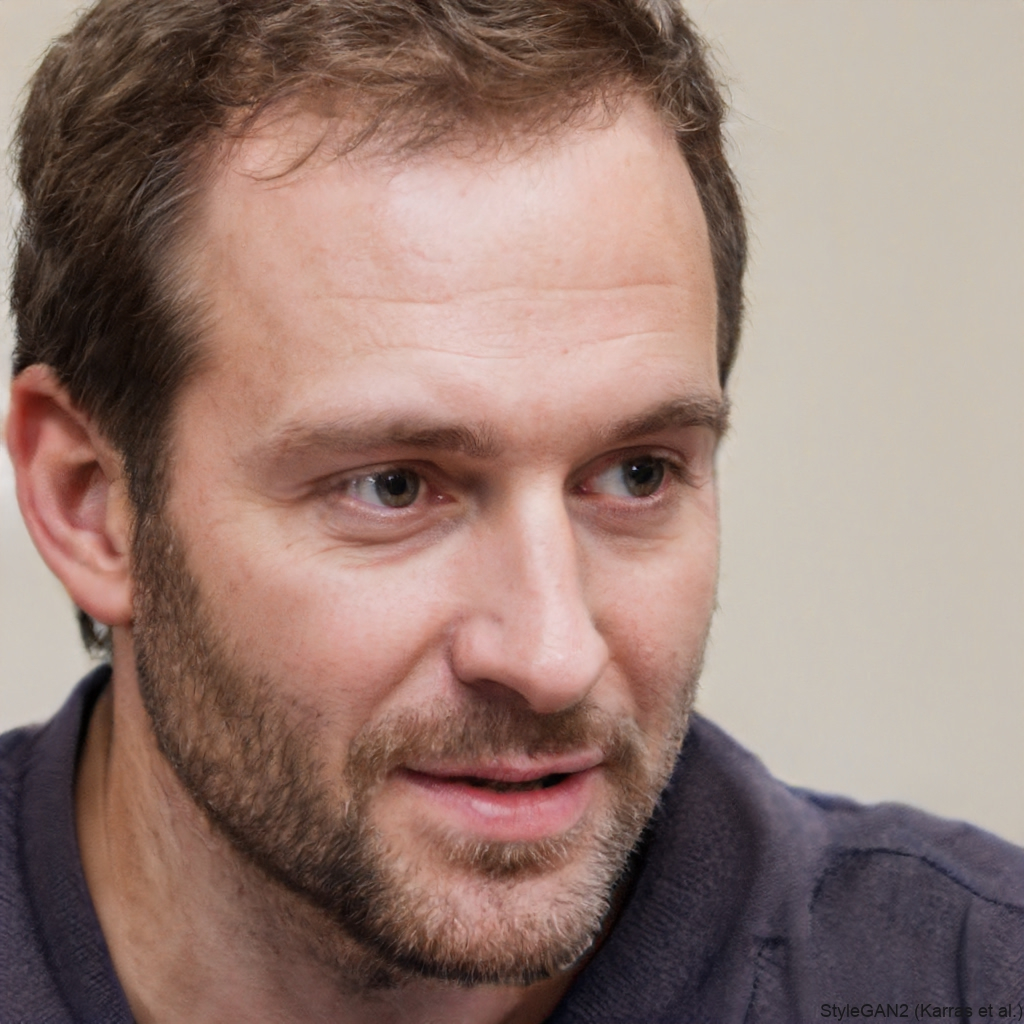
\includegraphics[width=0.25\textwidth]{martin} \\
        Name       & Martin Jensen                                  \\
        Age        & 34 years old                                   \\
        Occupation & Factory worker                                 \\
        What's important & For Martin it is important to live a carefree life.
        He has a family and friends at work, so he's pretty happy with himself. \\
        Current problem & Martin drives a gas car to work, but he wants to change that for the sake of the environment.
        He has gotten used to the comfort of his car, but can't afford an electric car.
        He wonders if public transport could match that. \\
        Potential solution & We would want to make a program, where Martin can figure out what forms of public transport are
        most comfortable and most climate friendly. \\
        \hline
    \end{tabularx}
    \caption{Persona: Martin.}
    % textidote: ignore begin
    \label{fig:persona_martin}
    % textidote: ignore end
\end{figure}
